\chapterimage{chapter_head_1.png}

\chapter{Informierte Suche}
\section{Beispiel}

Wir wollen nun den $\text{A}^*$ Algorithmus an einem Beispiel anwenden.
Sei dazu der Graph $G$ und die Heuristik $h$ durch
\fbox{
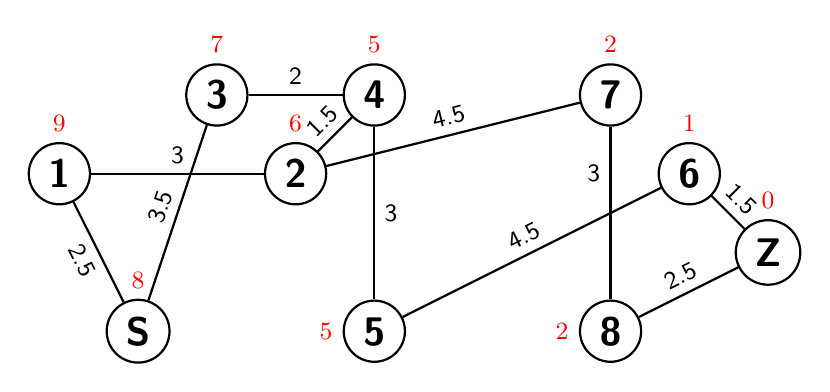
\begin{tikzpicture}[auto, node distance=2cm, every loop/.style={},
                    thick,main node/.style={circle,draw,font=\sffamily\Large\bfseries}]

  \node[main node, label={\color{red}\small 9}] (1) at (1, 3) {1};
  \node[main node, label={\color{red}\small 6}] (2) at (4, 3) {2};
  \node[main node, label={\color{red}\small 7}] (3) at (3, 4) {3};
  \node[main node, label={\color{red}\small 5}] (4) at (5, 4) {4};
  \node[main node, label=left:{\color{red}\small 5}] (5) at (5, 1) {5};
  \node[main node, label={\color{red}\small 1}] (6) at (9, 3) {6};
  \node[main node, label={\color{red}\small 2}] (7) at (8, 4) {7};
  \node[main node, label=left:{\color{red}\small 2}] (8) at (8, 1) {8};
  \node[main node, label={\color{red}\small 8}] (9) at (2, 1) {S};
  \node[main node, label={\color{red}\small 0}] (10) at (10, 2) {Z};

  \path[every node/.style={font=\sffamily\small}]
  (9) edge node [sloped, below] {2.5} (1)
  (1) edge node [sloped] {3} (2)
  (2) edge node [sloped, above] {4.5} (7)
  (7) edge node [left, yshift=0.5cm] {3} (8)
  (8) edge node [sloped, above] {2.5} (10)
  (9) edge node [sloped] {3.5} (3)
  (3) edge node [sloped] {2} (4)
  (4) edge node [right] {3} (5)
  (5) edge node [sloped] {4.5} (6)
  (6) edge node [sloped, above] {1.5} (10)
  (4) edge node [sloped, above] {1.5} (2);

\end{tikzpicture}}\vspace{5pt}\\
gegeben. Wir wollen einen Weg von $S$ nach $Z$ suchen. Man erhält Folgendes:
(hierbei ist eine Zahl im Knoten rot, falls er in der Extended-List
ist, grün wenn er gerade expandiert wird und gelb falls er auf der Open-List
ist):\vspace{5pt}\\
\fbox{
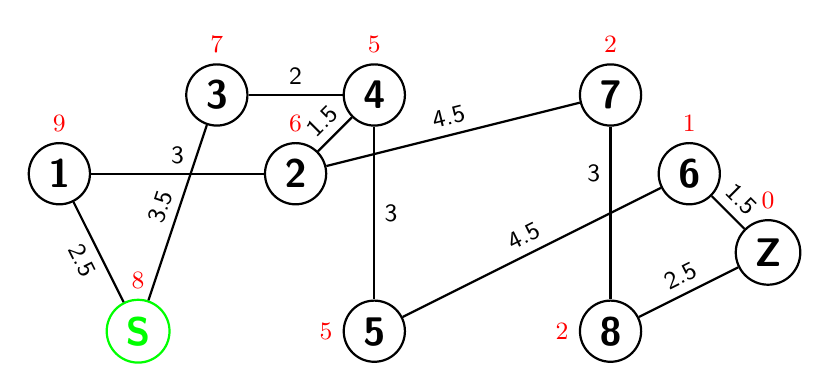
\begin{tikzpicture}[auto, node distance=2cm, every loop/.style={},
                    thick,main node/.style={circle,draw,font=\sffamily\Large\bfseries}]

  \node[main node, label={\color{red}\small 9}] (1) at (1, 3) {1};
  \node[main node, label={\color{red}\small 6}] (2) at (4, 3) {2};
  \node[main node, label={\color{red}\small 7}] (3) at (3, 4) {3};
  \node[main node, label={\color{red}\small 5}] (4) at (5, 4) {4};
  \node[main node, label=left:{\color{red}\small 5}] (5) at (5, 1) {5};
  \node[main node, label={\color{red}\small 1}] (6) at (9, 3) {6};
  \node[main node, label={\color{red}\small 2}] (7) at (8, 4) {7};
  \node[main node, label=left:{\color{red}\small 2}] (8) at (8, 1) {8};
  \node[main node, color=green, label={\color{red}\small 8}] (9) at (2, 1) {S};
  \node[main node, label={\color{red}\small 0}] (10) at (10, 2) {Z};

  \path[every node/.style={font=\sffamily\small}]
  (9) edge node [sloped, below] {2.5} (1)
  (1) edge node [sloped] {3} (2)
  (2) edge node [sloped, above] {4.5} (7)
  (7) edge node [left, yshift=0.5cm] {3} (8)
  (8) edge node [sloped, above] {2.5} (10)
  (9) edge node [sloped] {3.5} (3)
  (3) edge node [sloped] {2} (4)
  (4) edge node [right] {3} (5)
  (5) edge node [sloped] {4.5} (6)
  (6) edge node [sloped, above] {1.5} (10)
  (4) edge node [sloped, above] {1.5} (2);

\end{tikzpicture}}
\hfill
\fbox{\begin{minipage}[b][4.27cm][t]{0.34\textwidth}
    \begin{tabular}{|l|r|}
      Queue & Prio\\
      (S) & 8\\
      \phantom{(S, 3, 4, 5, 6, Z)} & \phantom{14.5}
    \end{tabular}
\end{minipage}}\vspace{5pt}\\
\fbox{
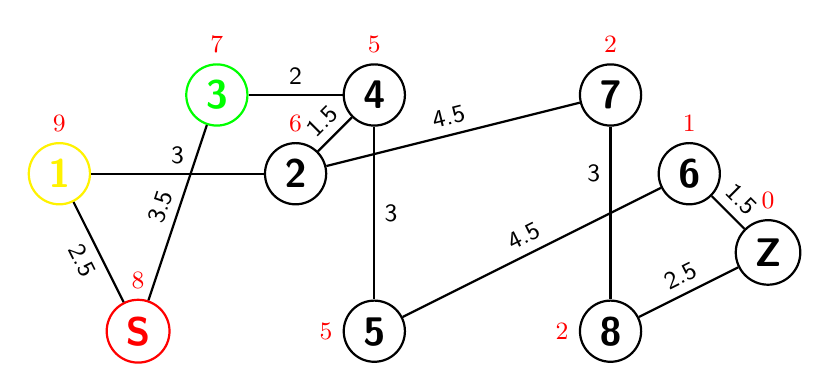
\begin{tikzpicture}[auto, node distance=2cm, every loop/.style={},
                    thick,main node/.style={circle,draw,font=\sffamily\Large\bfseries}]

  \node[main node, color=yellow, label={\color{red}\small 9}] (1) at (1, 3) {1};
  \node[main node, label={\color{red}\small 6}] (2) at (4, 3) {2};
  \node[main node, color=green, label={\color{red}\small 7}] (3) at (3, 4) {3};
  \node[main node, label={\color{red}\small 5}] (4) at (5, 4) {4};
  \node[main node, label=left:{\color{red}\small 5}] (5) at (5, 1) {5};
  \node[main node, label={\color{red}\small 1}] (6) at (9, 3) {6};
  \node[main node, label={\color{red}\small 2}] (7) at (8, 4) {7};
  \node[main node, label=left:{\color{red}\small 2}] (8) at (8, 1) {8};
  \node[main node, color=red, label={\color{red}\small 8}] (9) at (2, 1) {S};
  \node[main node, label={\color{red}\small 0}] (10) at (10, 2) {Z};

  \path[every node/.style={font=\sffamily\small}]
  (9) edge node [sloped, below] {2.5} (1)
  (1) edge node [sloped] {3} (2)
  (2) edge node [sloped, above] {4.5} (7)
  (7) edge node [left, yshift=0.5cm] {3} (8)
  (8) edge node [sloped, above] {2.5} (10)
  (9) edge node [sloped] {3.5} (3)
  (3) edge node [sloped] {2} (4)
  (4) edge node [right] {3} (5)
  (5) edge node [sloped] {4.5} (6)
  (6) edge node [sloped, above] {1.5} (10)
  (4) edge node [sloped, above] {1.5} (2);

\end{tikzpicture}}\hfill
\fbox{\begin{minipage}[b][4.27cm][t]{0.34\textwidth}
    \begin{tabular}{|l|r|}
      Queue & Prio\\
      (S, 3) & 10\\
      (S, 1) & 11.5\\
      \phantom{(S, 3, 4, 5, 6, Z)} & \phantom{14.5}
    \end{tabular}
\end{minipage}}
\vspace{5pt}\\
\fbox{
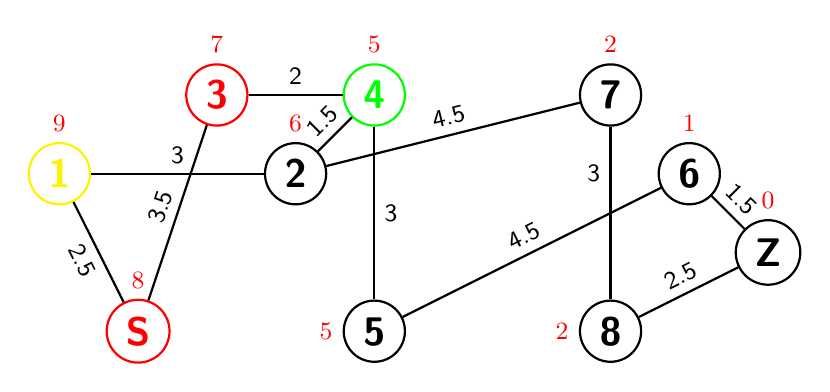
\begin{tikzpicture}[auto, node distance=2cm, every loop/.style={},
                    thick,main node/.style={circle,draw,font=\sffamily\Large\bfseries}]

  \node[main node, color=yellow, label={\color{red}\small 9}] (1) at (1, 3) {1};
  \node[main node, label={\color{red}\small 6}] (2) at (4, 3) {2};
  \node[main node, color=red, label={\color{red}\small 7}] (3) at (3, 4) {3};
  \node[main node, color=green, label={\color{red}\small 5}] (4) at (5, 4) {4};
  \node[main node, label=left:{\color{red}\small 5}] (5) at (5, 1) {5};
  \node[main node, label={\color{red}\small 1}] (6) at (9, 3) {6};
  \node[main node, label={\color{red}\small 2}] (7) at (8, 4) {7};
  \node[main node, label=left:{\color{red}\small 2}] (8) at (8, 1) {8};
  \node[main node, color=red, label={\color{red}\small 8}] (9) at (2, 1) {S};
  \node[main node, label={\color{red}\small 0}] (10) at (10, 2) {Z};

  \path[every node/.style={font=\sffamily\small}]
  (9) edge node [sloped, below] {2.5} (1)
  (1) edge node [sloped] {3} (2)
  (2) edge node [sloped, above] {4.5} (7)
  (7) edge node [left, yshift=0.5cm] {3} (8)
  (8) edge node [sloped, above] {2.5} (10)
  (9) edge node [sloped] {3.5} (3)
  (3) edge node [sloped] {2} (4)
  (4) edge node [right] {3} (5)
  (5) edge node [sloped] {4.5} (6)
  (6) edge node [sloped, above] {1.5} (10)
  (4) edge node [sloped, above] {1.5} (2);

\end{tikzpicture}}\hfill
\fbox{\begin{minipage}[b][4.27cm][t]{0.34\textwidth}
    \begin{tabular}{|l|r|}
      Queue & Prio\\
      (S, 3, 4) & 10\\
      (S, 1) & 11.5\\
      \phantom{(S, 3, 4, 5, 6, Z)} & \phantom{14.5}
    \end{tabular}
\end{minipage}}\vspace{5pt}\\
\fbox{
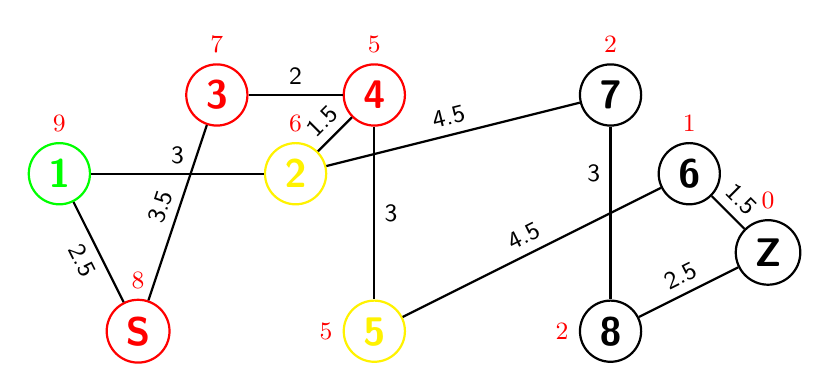
\begin{tikzpicture}[auto, node distance=2cm, every loop/.style={},
                    thick,main node/.style={circle,draw,font=\sffamily\Large\bfseries}]

  \node[main node, color=green, label={\color{red}\small 9}] (1) at (1, 3) {1};
  \node[main node, color=yellow, label={\color{red}\small 6}] (2) at (4, 3) {2};
  \node[main node, color=red, label={\color{red}\small 7}] (3) at (3, 4) {3};
  \node[main node, color=red, label={\color{red}\small 5}] (4) at (5, 4) {4};
  \node[main node, color=yellow, label=left:{\color{red}\small 5}] (5) at (5, 1) {5};
  \node[main node, label={\color{red}\small 1}] (6) at (9, 3) {6};
  \node[main node, label={\color{red}\small 2}] (7) at (8, 4) {7};
  \node[main node, label=left:{\color{red}\small 2}] (8) at (8, 1) {8};
  \node[main node, color=red, label={\color{red}\small 8}] (9) at (2, 1) {S};
  \node[main node, label={\color{red}\small 0}] (10) at (10, 2) {Z};

  \path[every node/.style={font=\sffamily\small}]
  (9) edge node [sloped, below] {2.5} (1)
  (1) edge node [sloped] {3} (2)
  (2) edge node [sloped, above] {4.5} (7)
  (7) edge node [left, yshift=0.5cm] {3} (8)
  (8) edge node [sloped, above] {2.5} (10)
  (9) edge node [sloped] {3.5} (3)
  (3) edge node [sloped] {2} (4)
  (4) edge node [right] {3} (5)
  (5) edge node [sloped] {4.5} (6)
  (6) edge node [sloped, above] {1.5} (10)
  (4) edge node [sloped, above] {1.5} (2);

\end{tikzpicture}}\hfill
\fbox{\begin{minipage}[b][4.27cm][t]{0.34\textwidth}
    \begin{tabular}{|l|r|}
      Queue & Prio\\
      (S, 1) & 11.5\\
      (S, 3, 4, 2) & 13\\
      (S, 3, 4, 5) & 13.5\\
      \phantom{(S, 3, 4, 5, 6, Z)} & \phantom{14.5}
    \end{tabular}
\end{minipage}}\vspace{5pt}\\
\fbox{
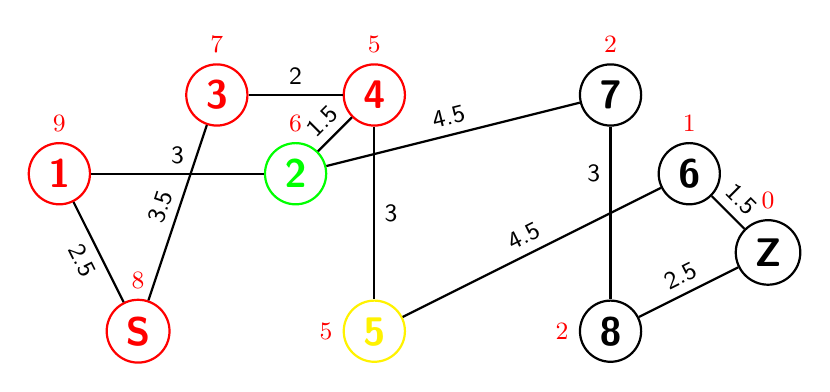
\begin{tikzpicture}[auto, node distance=2cm, every loop/.style={},
                    thick,main node/.style={circle,draw,font=\sffamily\Large\bfseries}]

  \node[main node, color=red, label={\color{red}\small 9}] (1) at (1, 3) {1};
  \node[main node, color=green, label={\color{red}\small 6}] (2) at (4, 3) {2};
  \node[main node, color=red, label={\color{red}\small 7}] (3) at (3, 4) {3};
  \node[main node, color=red, label={\color{red}\small 5}] (4) at (5, 4) {4};
  \node[main node, color=yellow, label=left:{\color{red}\small 5}] (5) at (5, 1) {5};
  \node[main node, label={\color{red}\small 1}] (6) at (9, 3) {6};
  \node[main node, label={\color{red}\small 2}] (7) at (8, 4) {7};
  \node[main node, label=left:{\color{red}\small 2}] (8) at (8, 1) {8};
  \node[main node, color=red, label={\color{red}\small 8}] (9) at (2, 1) {S};
  \node[main node, label={\color{red}\small 0}] (10) at (10, 2) {Z};

  \path[every node/.style={font=\sffamily\small}]
  (9) edge node [sloped, below] {2.5} (1)
  (1) edge node [sloped] {3} (2)
  (2) edge node [sloped, above] {4.5} (7)
  (7) edge node [left, yshift=0.5cm] {3} (8)
  (8) edge node [sloped, above] {2.5} (10)
  (9) edge node [sloped] {3.5} (3)
  (3) edge node [sloped] {2} (4)
  (4) edge node [right] {3} (5)
  (5) edge node [sloped] {4.5} (6)
  (6) edge node [sloped, above] {1.5} (10)
  (4) edge node [sloped, above] {1.5} (2);

\end{tikzpicture}}\hfill
\fbox{\begin{minipage}[b][4.27cm][t]{0.34\textwidth}
    \begin{tabular}{|l|r|}
      Queue & Prio\\
      (S, 1, 2) & 11.5\\
      (S, 3, 4, 2) & 13\\
      (S, 3, 4, 5) & 13.5\\
      \phantom{(S, 3, 4, 5, 6, Z)} & \phantom{14.5}
    \end{tabular}
\end{minipage}}\vspace{5pt}\\
\fbox{
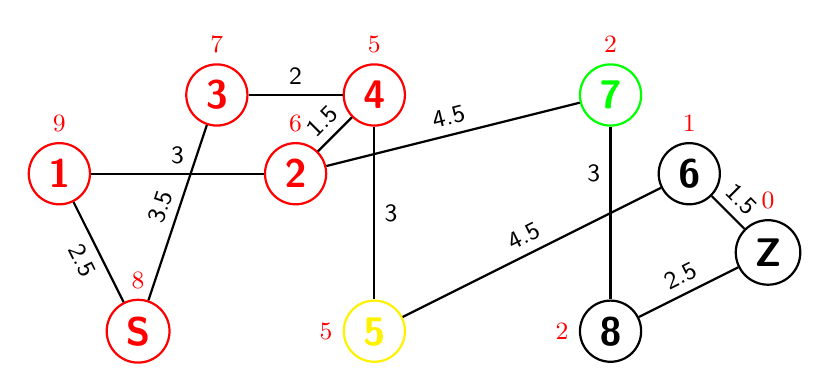
\begin{tikzpicture}[auto, node distance=2cm, every loop/.style={},
                    thick,main node/.style={circle,draw,font=\sffamily\Large\bfseries}]

  \node[main node, color=red, label={\color{red}\small 9}] (1) at (1, 3) {1};
  \node[main node, color=red, label={\color{red}\small 6}] (2) at (4, 3) {2};
  \node[main node, color=red, label={\color{red}\small 7}] (3) at (3, 4) {3};
  \node[main node, color=red, label={\color{red}\small 5}] (4) at (5, 4) {4};
  \node[main node, color=yellow, label=left:{\color{red}\small 5}] (5) at (5, 1) {5};
  \node[main node, label={\color{red}\small 1}] (6) at (9, 3) {6};
  \node[main node, color=green, label={\color{red}\small 2}] (7) at (8, 4) {7};
  \node[main node, label=left:{\color{red}\small 2}] (8) at (8, 1) {8};
  \node[main node, color=red, label={\color{red}\small 8}] (9) at (2, 1) {S};
  \node[main node, label={\color{red}\small 0}] (10) at (10, 2) {Z};

  \path[every node/.style={font=\sffamily\small}]
  (9) edge node [sloped, below] {2.5} (1)
  (1) edge node [sloped] {3} (2)
  (2) edge node [sloped, above] {4.5} (7)
  (7) edge node [left, yshift=0.5cm] {3} (8)
  (8) edge node [sloped, above] {2.5} (10)
  (9) edge node [sloped] {3.5} (3)
  (3) edge node [sloped] {2} (4)
  (4) edge node [right] {3} (5)
  (5) edge node [sloped] {4.5} (6)
  (6) edge node [sloped, above] {1.5} (10)
  (4) edge node [sloped, above] {1.5} (2);

\end{tikzpicture}}\hfill
\fbox{\begin{minipage}[b][4.27cm][t]{0.34\textwidth}
    \begin{tabular}{|l|r|}
      Queue & Prio\\
      (S, 1, 2, 7) & 12\\
      (S, 3, 4, 2) & 13\\
      (S, 3, 4, 5) & 13.5\\
      \phantom{(S, 3, 4, 5, 6, Z)} & \phantom{14.5}
    \end{tabular}
\end{minipage}}\vspace{5pt}\\
\fbox{
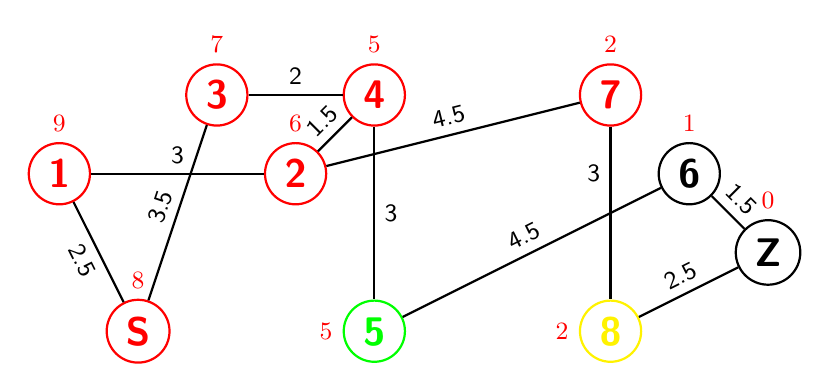
\begin{tikzpicture}[auto, node distance=2cm, every loop/.style={},
                    thick,main node/.style={circle,draw,font=\sffamily\Large\bfseries}]

  \node[main node, color=red, label={\color{red}\small 9}] (1) at (1, 3) {1};
  \node[main node, color=red, label={\color{red}\small 6}] (2) at (4, 3) {2};
  \node[main node, color=red, label={\color{red}\small 7}] (3) at (3, 4) {3};
  \node[main node, color=red, label={\color{red}\small 5}] (4) at (5, 4) {4};
  \node[main node, color=green, label=left:{\color{red}\small 5}] (5) at (5, 1) {5};
  \node[main node, label={\color{red}\small 1}] (6) at (9, 3) {6};
  \node[main node, color=red, label={\color{red}\small 2}] (7) at (8, 4) {7};
  \node[main node, color=yellow, label=left:{\color{red}\small 2}] (8) at (8, 1) {8};
  \node[main node, color=red, label={\color{red}\small 8}] (9) at (2, 1) {S};
  \node[main node, label={\color{red}\small 0}] (10) at (10, 2) {Z};

  \path[every node/.style={font=\sffamily\small}]
  (9) edge node [sloped, below] {2.5} (1)
  (1) edge node [sloped] {3} (2)
  (2) edge node [sloped, above] {4.5} (7)
  (7) edge node [left, yshift=0.5cm] {3} (8)
  (8) edge node [sloped, above] {2.5} (10)
  (9) edge node [sloped] {3.5} (3)
  (3) edge node [sloped] {2} (4)
  (4) edge node [right] {3} (5)
  (5) edge node [sloped] {4.5} (6)
  (6) edge node [sloped, above] {1.5} (10)
  (4) edge node [sloped, above] {1.5} (2);

\end{tikzpicture}}\hfill
\fbox{\begin{minipage}[b][4.27cm][t]{0.34\textwidth}
    \begin{tabular}{|l|r|}
      Queue & Prio\\
      (S, 3, 4, 5) & 13.5\\
      (S, 1, 2, 7, 8) & 15\\
      \phantom{(S, 3, 4, 5, 6, Z)} & \phantom{14.5}
    \end{tabular}\\
    Der Weg $(S, 3, 4, 2)$ wurde entfernt, da $2$ schon in der Closed-List ist.
\end{minipage}}\vspace{5pt}\\
\fbox{
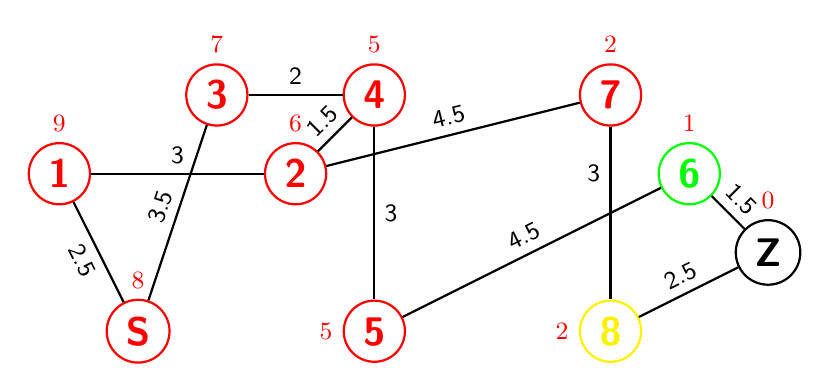
\begin{tikzpicture}[auto, node distance=2cm, every loop/.style={},
                    thick,main node/.style={circle,draw,font=\sffamily\Large\bfseries}]

  \node[main node, color=red, label={\color{red}\small 9}] (1) at (1, 3) {1};
  \node[main node, color=red, label={\color{red}\small 6}] (2) at (4, 3) {2};
  \node[main node, color=red, label={\color{red}\small 7}] (3) at (3, 4) {3};
  \node[main node, color=red, label={\color{red}\small 5}] (4) at (5, 4) {4};
  \node[main node, color=red, label=left:{\color{red}\small 5}] (5) at (5, 1) {5};
  \node[main node, color=green, label={\color{red}\small 1}] (6) at (9, 3) {6};
  \node[main node, color=red, label={\color{red}\small 2}] (7) at (8, 4) {7};
  \node[main node, color=yellow, label=left:{\color{red}\small 2}] (8) at (8, 1) {8};
  \node[main node, color=red, label={\color{red}\small 8}] (9) at (2, 1) {S};
  \node[main node, label={\color{red}\small 0}] (10) at (10, 2) {Z};

  \path[every node/.style={font=\sffamily\small}]
  (9) edge node [sloped, below] {2.5} (1)
  (1) edge node [sloped] {3} (2)
  (2) edge node [sloped, above] {4.5} (7)
  (7) edge node [left, yshift=0.5cm] {3} (8)
  (8) edge node [sloped, above] {2.5} (10)
  (9) edge node [sloped] {3.5} (3)
  (3) edge node [sloped] {2} (4)
  (4) edge node [right] {3} (5)
  (5) edge node [sloped] {4.5} (6)
  (6) edge node [sloped, above] {1.5} (10)
  (4) edge node [sloped, above] {1.5} (2);

\end{tikzpicture}}\hfill
\fbox{\begin{minipage}[b][4.27cm][t]{0.34\textwidth}
    \begin{tabular}{|l|r|}
      Weg & Prio\\
      (S, 3, 4, 5, 6) & 14\\
      (S, 1, 2, 7, 8) & 15\\
      \phantom{(S, 3, 4, 5, 6, Z)} & \phantom{14.5}
    \end{tabular}
\end{minipage}}\vspace{5pt}\\
\fbox{
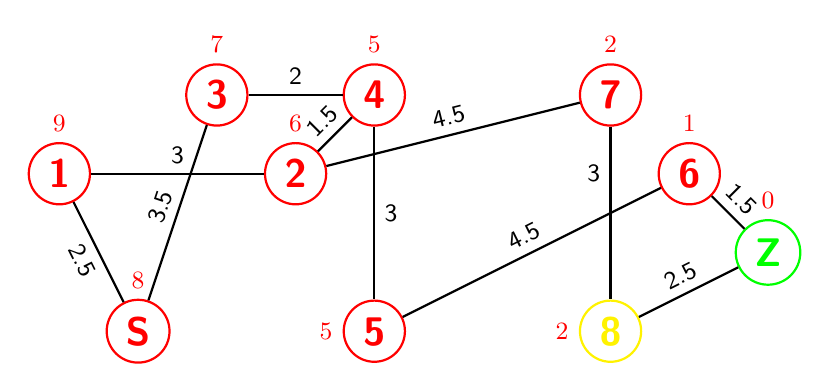
\begin{tikzpicture}[auto, node distance=2cm, every loop/.style={},
                    thick,main node/.style={circle,draw,font=\sffamily\Large\bfseries}]

  \node[main node, color=red, label={\color{red}\small 9}] (1) at (1, 3) {1};
  \node[main node, color=red, label={\color{red}\small 6}] (2) at (4, 3) {2};
  \node[main node, color=red, label={\color{red}\small 7}] (3) at (3, 4) {3};
  \node[main node, color=red, label={\color{red}\small 5}] (4) at (5, 4) {4};
  \node[main node, color=red, label=left:{\color{red}\small 5}] (5) at (5, 1) {5};
  \node[main node, color=red, label={\color{red}\small 1}] (6) at (9, 3) {6};
  \node[main node, color=red, label={\color{red}\small 2}] (7) at (8, 4) {7};
  \node[main node, color=yellow, label=left:{\color{red}\small 2}] (8) at (8, 1) {8};
  \node[main node, color=red, label={\color{red}\small 8}] (9) at (2, 1) {S};
  \node[main node, color=green, label={\color{red}\small 0}] (10) at (10, 2) {Z};

  \path[every node/.style={font=\sffamily\small}]
  (9) edge node [sloped, below] {2.5} (1)
  (1) edge node [sloped] {3} (2)
  (2) edge node [sloped, above] {4.5} (7)
  (7) edge node [left, yshift=0.5cm] {3} (8)
  (8) edge node [sloped, above] {2.5} (10)
  (9) edge node [sloped] {3.5} (3)
  (3) edge node [sloped] {2} (4)
  (4) edge node [right] {3} (5)
  (5) edge node [sloped] {4.5} (6)
  (6) edge node [sloped, above] {1.5} (10)
  (4) edge node [sloped, above] {1.5} (2);

\end{tikzpicture}}\hfill
\fbox{\begin{minipage}[b][4.27cm][t]{0.34\textwidth}
    \begin{tabular}{|l|r|}
      Weg & Prio\\
      (S, 3, 4, 5, 6, Z) & 14.5\\
      (S, 1, 2, 7, 8) & 15\\
      \phantom{(S, 3, 4, 5, 6, Z)} & \phantom{14.5}
    \end{tabular}\\
    Hier bricht Algorithmus ab, da $Z$ zu suchen war, und gibt
    $(S, 3, 4, 5, 6, Z)$ aus.
\end{minipage}}\vspace{5pt}\\
Somit ist $(S, 3, 4, 5, 6, Z)$ der kürzeste Weg von $S$ nach $Z$.
